\documentclass[a4paper, 12pt]{article}
\usepackage{config}

\usepackage{import}
\usepackage{xwatermark}
\newwatermark[allpages, scale=3, color=gray!20, angle=60, xpos=-10, ypos=10]{FA576}

\author{Renan Guedes}
\title{Relatório}

\begin{document}
	\begin{titlepage}
		\begin{center}
			\begin{large}
				\textbf{Universidade Estadual de Campinas}\\\vspace{1cm}
				\textbf{Faculdade de Engenharia Agrícola}\\
			\end{large}
			\vspace{10cm}
			\begin{Large}
				\uppercase{\textbf{Compressão Uniaxial}}\\
			\end{Large}
		\end{center}
		\vspace{5cm}
		\begin{large}
			\textbf{Nome:} Renan da Silva Guedes | 223979
		\end{large}
	\end{titlepage}
	
	\newpage
	
	\tableofcontents
	\listoffigures
	\listoftables
	
	\newpage
	
	\section{Introdução}
	
	O experimento realizado terá como base ensaios de compressão uniaxial em corpos de prova de batata inglesa. Tendo em vista a importância do conhecimento das características mecânicas de um produto, ao analisar os seus atributos de forma empírica, possibilita-se explorar esses elementos na elaboração de projetos, com base em seu comportamento, peculiaridades e limitações. 
	
	\section{Objetivo}
	
	Determinação do módulo de elasticidade (Módulo de \textit{Young}).
	
	\section{Materiais e Métodos}
	
	Para a realização do experimento foi feito uso de batatas inglesas, cortador de batata cilíndrico, paquímetro digital, máquina universal de ensaios e \textit{software} para aquisição dos dados.

	A figura \ref{potato} ilustra os procedimentos adotados na primeira parte do experimento. Inicialmente, fazendo uso das batatas, submeteu-se as mesmas aos cortadores cilíndricos, de modo a obter corpos de prova uniformes. Feito isso, com o auxílio de um paquímetro, foram coletados os valores de altura e diâmetro.
	
	Dessa forma, repetiu-se o procedimento para 15 corpos de prova e todos os valores foram anotados como mostra a tabela \ref{data}. Logo em seguida, os 15 corpos de prova foram divididos em três grupos. Cada grupo de 5 foi ensaiado a uma determinada velocidade como também mostra a tabela \ref{data}.
	
	Ao longo da realização dos ensaios, com o auxílio do \textit{software} para aquisição de dados, foi feito o armazenamento dos valores de força medidos (F, em \SI{}{\kilo gf}) pela célula de carga.
	
	Em seguida, foram construídos os gráficos da tensão ($\sigma$) em função da deformação do corpo ($\epsilon$), como é visto nas figuras \ref{fig:g1}, \ref{fig:g2} e \ref{fig:g3}. Com base no comportamento das curvas, foi realizado o ajuste da reta que melhor se adéqua ao trecho de menor variação adotado para o conjunto de 5 curvas em cada parte. Desta maneira, após construir as retas, aplicando o comando \texttt{Fit} do \textit{Wolfram Mathematica} foram obtidas as equações de reta que apresentam como propriedade o coeficiente angular igual ao módulo de elasticidade médio procurado.
	
	Por fim, com os valores do módulo de elasticidade obtidos (E$_{1}$, E$_{2}$, E$_{3}$) foi construído o gráfico que os relaciona com a velocidade de deformação aplicada aos corpos de prova ($v_{1}$, $v_{2}$, $v_{3}$), como é visto na figura \ref{fig:g4}. 
	
	\section{Resultados e discussão}
	
	A partir dos gráficos obtidos (Figuras \ref{fig:g1}, \ref{fig:g2} e \ref{fig:g3}), nota-se que ao elevar a velocidade de deformação dos corpos de prova cilíndricos ocorre elevação nos valores de módulo de elasticidade (Figura \ref{fig:g4}). 
	
	Na primeira parte do experimento, sob velocidade de \SI{.5}{\milli\meter/\second}, foi obtido um valor de $\textrm{E}_{1}=\SI{3.22}{\mega\pascal}$ com base no ajuste realizado. Na segunda etapa, a \SI{.8}{\milli\meter/\second} o comportamento mecânico da batata inglesa ocasionou aumento de \SI{.32}{\mega\pascal} ($\textrm{E}_{2}=\SI{3.54}{\mega\pascal}$) e, por fim, na bateria final ($v_{3}=\SI{1.2}{\milli\meter/\second}$), o valor de $\textrm{E}$ foi novamente incrementado levando a um $\textrm{E}_{3}=\SI{3.77}{\mega\pascal}$. 
	
	\section{Conclusão}
	
	A partir do ensaio realizado, nota-se que ao aplicar cargas mais rapidamente aos corpos de prova de batata inglesa, a mesma apresentou uma elevação do módulo de elasticidade como foi discutido. Dessa forma, conclui-se que deformações quando empregadas num menor intervalo de tempo ocasionam aumento nas tensões normais sentidas pelo corpo empregado no ensaio. 

	\newpage
	\section{Anexos}

	\begin{figure}[h!]
		\centering
		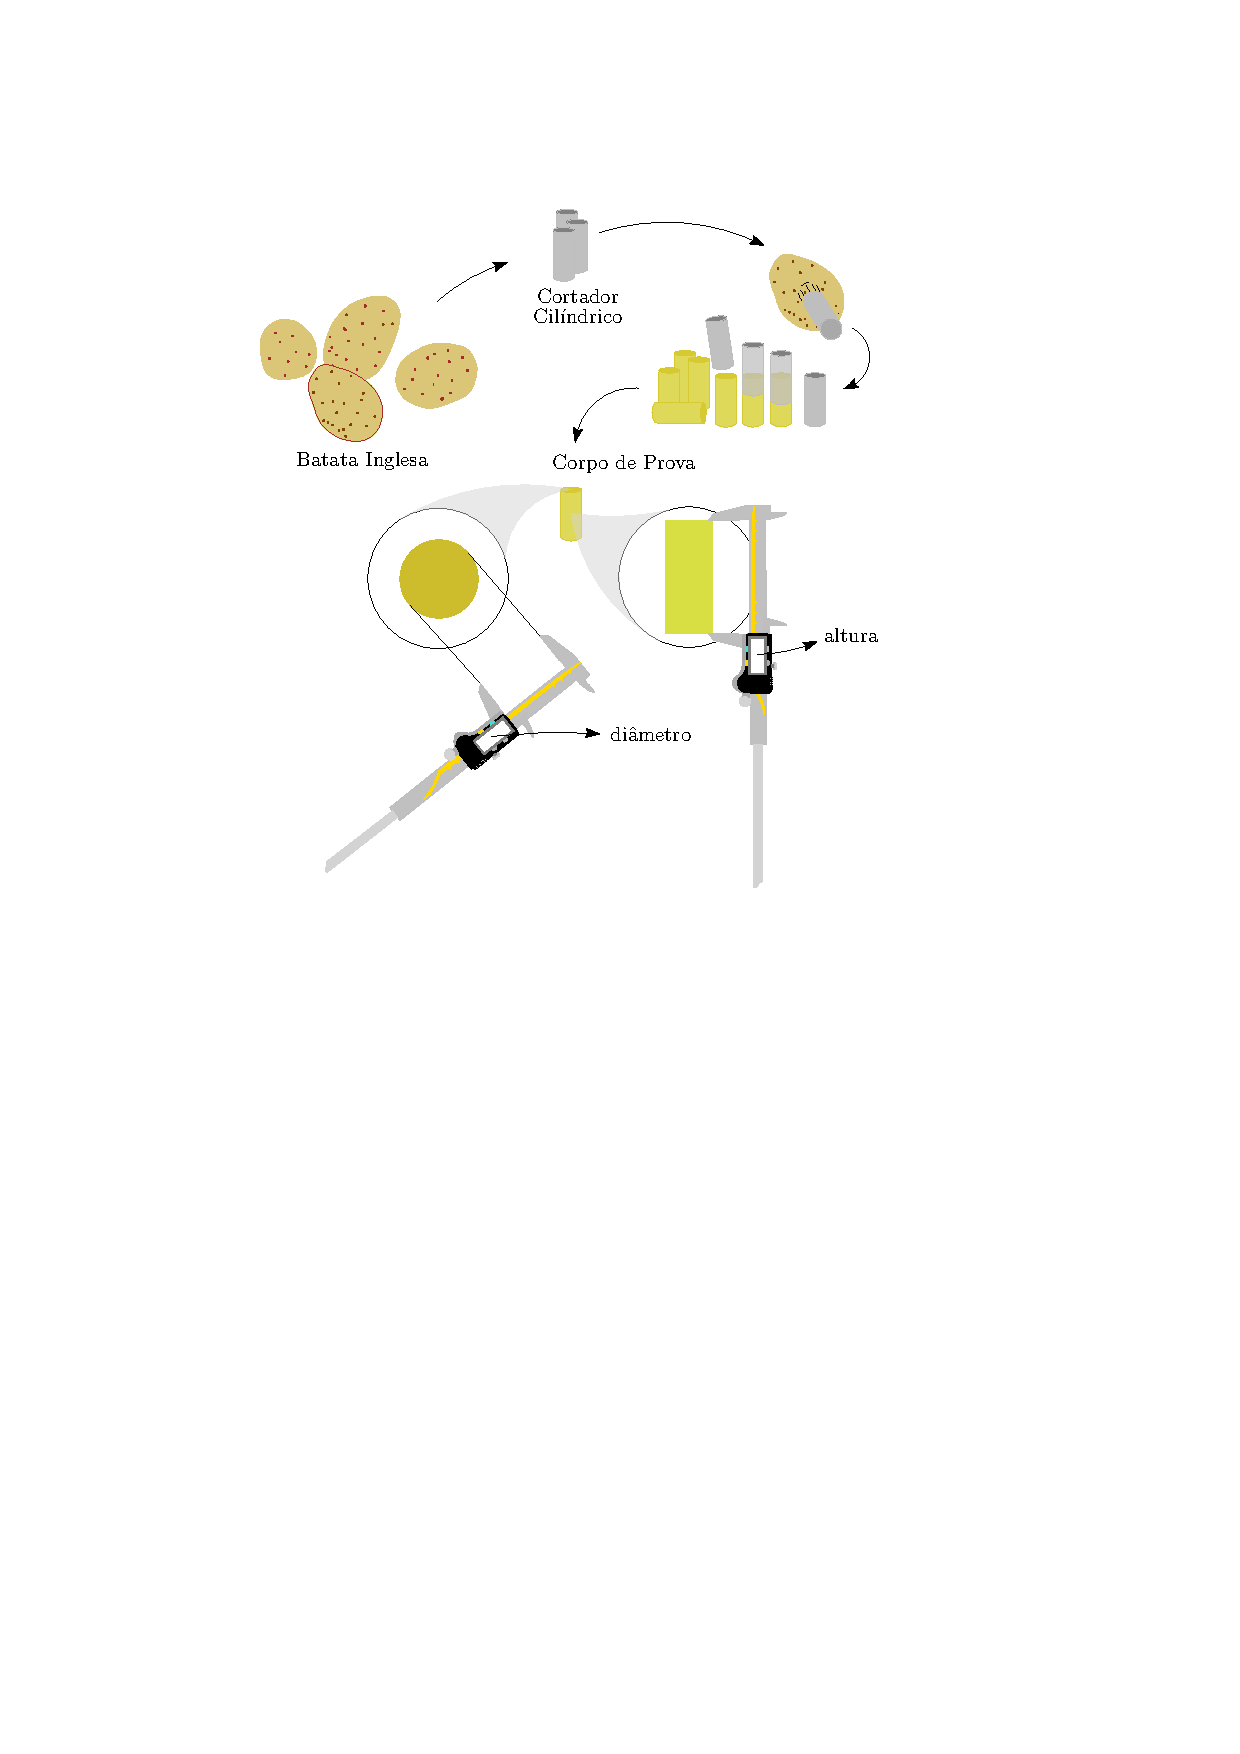
\includegraphics[scale=1.1]{sections/images/potato_diagram}
		\caption{Elaboração do corpo de prova e execução das medidas de diâmetro (D) e e altura (h) do mesmo.}
		\label{potato}
	\end{figure}
	
	\begin{figure}[h!]
		\centering
		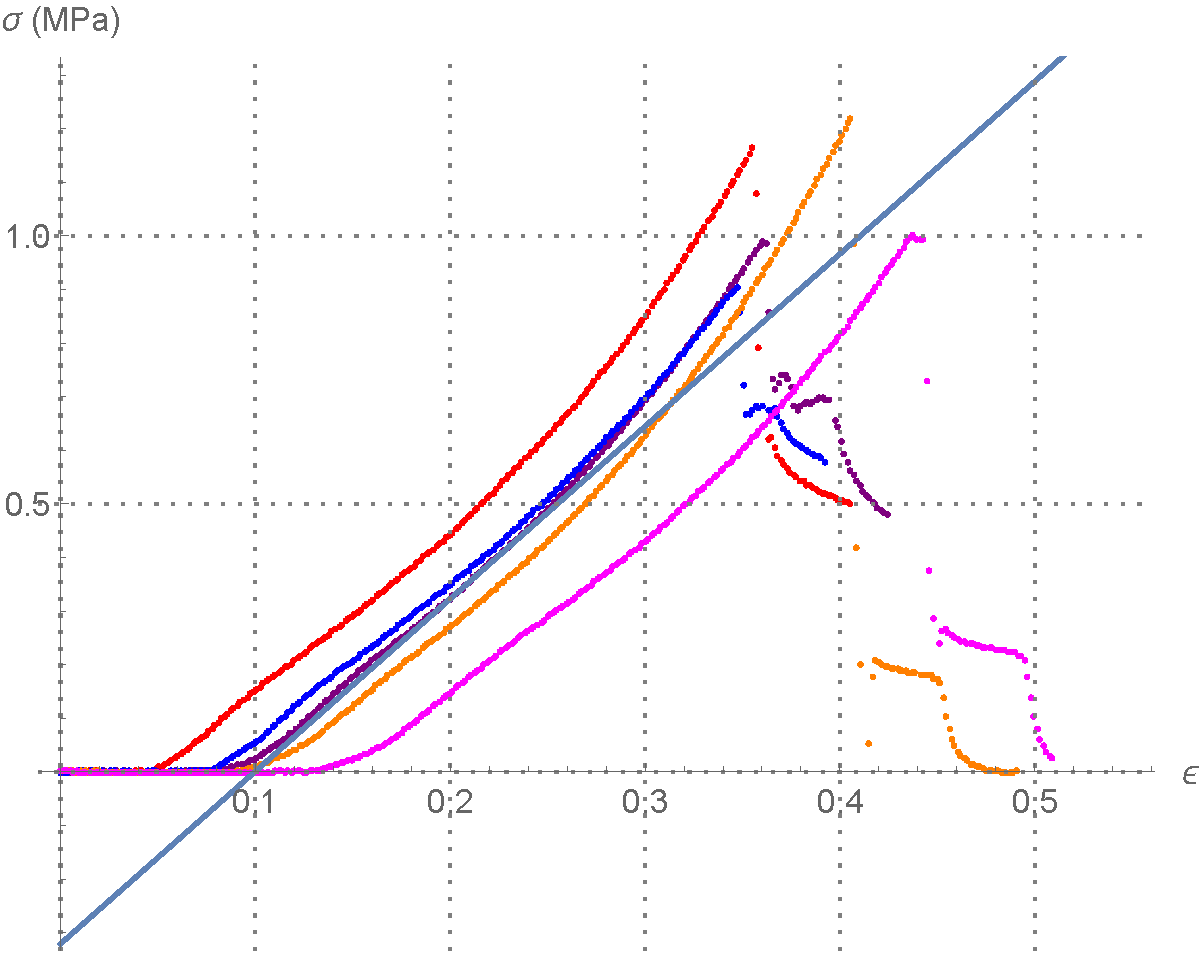
\includegraphics[width=0.65\linewidth]{sections/images/g1}
		\caption{Gráfico da tensão ($\sigma$, em \SI{}{\mega\pascal}) em função da deformação ($\epsilon$) sob compressão a \SI{.5}{\milli\meter/\second}}
		\label{fig:g1}
	\end{figure}
	
	\begin{figure}[h!]
		\centering
		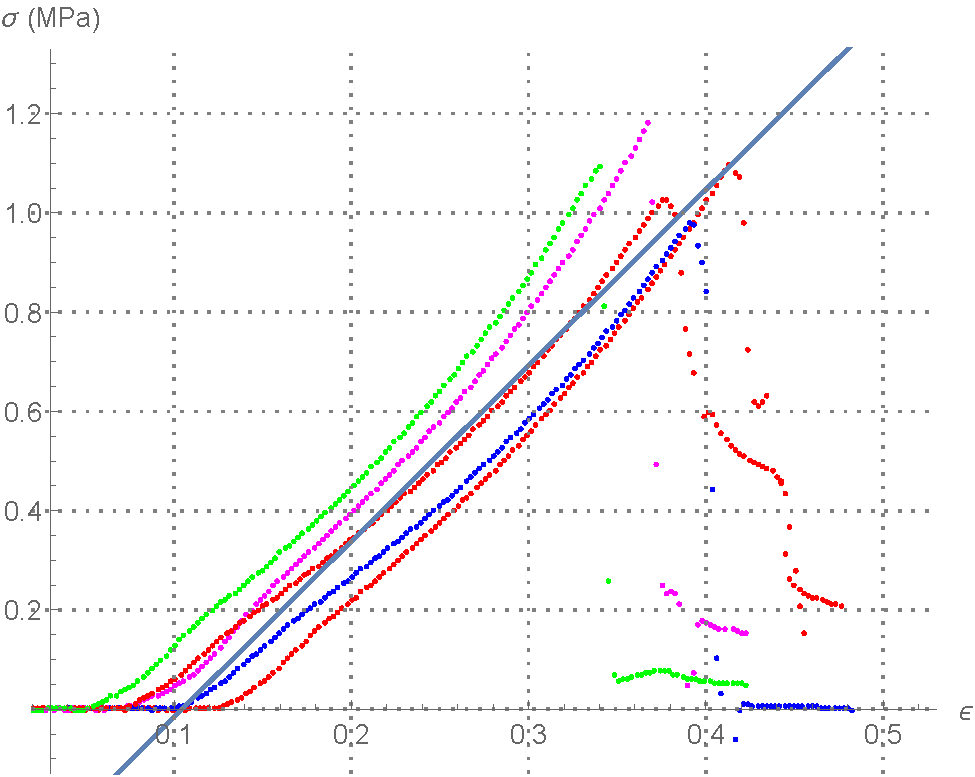
\includegraphics[width=0.65\linewidth]{sections/images/g2}
		\caption{Gráfico da tensão ($\sigma$, em \SI{}{\mega\pascal}) em função da deformação ($\epsilon$) sob compressão a \SI{.8}{\milli\meter/\second}}
		\label{fig:g2}
	\end{figure}
	
	\begin{figure}[h!]
		\centering
		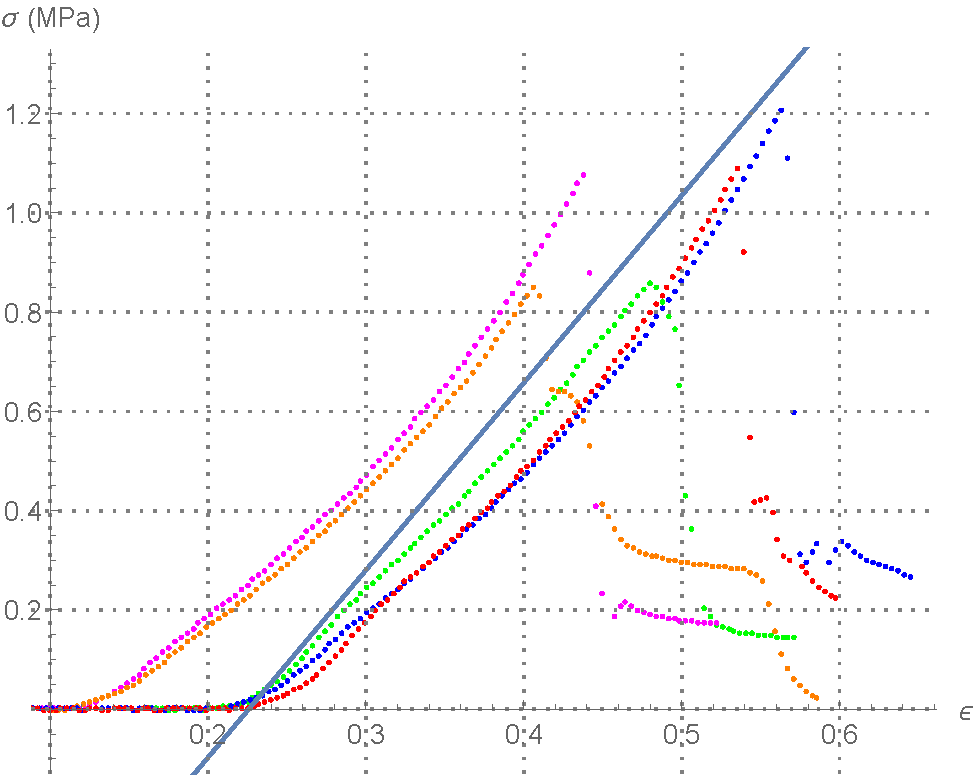
\includegraphics[width=0.65\linewidth]{sections/images/g3}
		\caption{Gráfico da tensão ($\sigma$, em \SI{}{\mega\pascal}) em função da deformação ($\epsilon$) sob compressão a \SI{1.2}{\milli\meter/\second}}
		\label{fig:g3}
	\end{figure}

	\begin{figure}[h!]
		\centering
		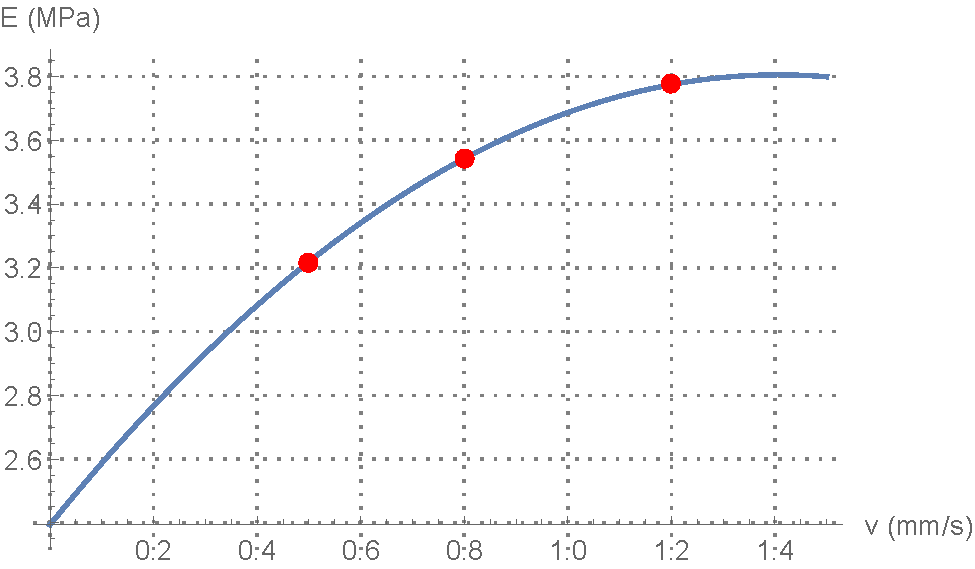
\includegraphics[width=0.65\linewidth]{sections/images/g4}
		\caption{Comportamento do módulo de elasticidade médio do corpo de prova sob diferentes velocidades na compressão.}
		\label{fig:g4}
	\end{figure}

	\import{sections/tables}{data}
	
	\import{sections/tables}{deviation}
	
\end{document}